\documentclass[12pt]{article}

% Load packages
\usepackage{cite}              % Make references as [1-4], not [1,2,3,4]
\usepackage{url}              	% Formatting web addresses
\usepackage{ifthen}           	% Conditional
\usepackage{multicol}			% Multi-column pages
\usepackage[utf8]{inputenc}   	% Unicode support
\usepackage{amsmath}           % Support for writing math formulas
\usepackage{amssymb}           % Support for writing math formulas
\usepackage{epsfig}            % Support separate PostScript files for figs
\usepackage{epstopdf}			% Converts eps figs to pdf
\usepackage{graphicx}			% Graphics functions
\usepackage[margin=0.1pt,font=footnotesize,labelfont=bf]{caption}
% \usepackage{caption}			% Styles figure captions
\usepackage{setspace}			% Provides line spacing environments
\usepackage{colortbl}
\usepackage[wide]{sidecap}		% Can typeset caption aside the figure, allows use of margin for figs wider than \textwidth.
\usepackage[square,sort,comma,numbers]{natbib}
% \usepackage[authoryear,square,comma,sort&compress]{natbib}
\usepackage{supertabular}		% Tables spanning multiple pages
\usepackage{comment}
\usepackage{lineno}
\urlstyle{rm}					% URL style
\usepackage{wrapfig}			% Wrap text around figures
\usepackage[FIGTOPCAP,nooneline]{subfigure}
\captionsetup{font={scriptsize},aboveskip=0pt}	% Styles figure captions
\usepackage{simplemargins}
\setallmargins{1.0in}         % Set all margins
% \setlength\bibsep{0pt}     % Single spaced bib
\date{} 
\doublespacing
% \singlespacing
\frenchspacing     % Eliminates double spaces between sentences

\makeatletter
\renewcommand\subsection{\@startsection
	{subsection}{2}{0mm}
	{-0.05in}
	{-0.5\baselineskip}
	{\normalfont\normalsize\bfseries}}
\renewcommand\subsubsection{\@startsection
	{subsubsection}{2}{0mm}
	{-0.05in}
	{-0.5\baselineskip}
	{\normalfont\normalsize\itshape}}
\renewcommand\section{\@startsection
	{subsection}{2}{0mm}
	{-0.2in}
	{0.05\baselineskip}
	{\normalfont\large\bfseries}}	
\renewcommand\paragraph{\@startsection
	{paragraph}{2}{0mm}
	{-0.05in}
	{-0.5\baselineskip}
	{\normalfont\normalsize\itshape}}
\makeatother

\newboolean{publ}

%Publication style settings
%\newenvironment{bmcformat}{\fussy\setboolean{publ}{true}}{\fussy}
\renewcommand{\rmdefault}{phv}\renewcommand{\sfdefault}{phv}
\renewcommand{\bibnumfmt}[1]{#1.}    % Change the number format in the ref list
\renewcommand{\figurename}{Fig.}     % Change Figure to Fig.

%%%%%%%%%%%%%%%%%%%%%%%%%%%%%%%%%%%%%%%%%%%%%%%%%%%%%%%%%%%%%%%%%%%%%
%%%%%%%%%%%%%%%%%%%%%%%%%%%%%%%%%%%%%%%%%%%%%%%%%%%%%%%%%%%%%%%%%%%%%

\begin{document}

%%%%%%%%%%%%%%%%%%%%%%%%%%%%%%%%%%%%%%%%%%%%%%%%%%%%%%%%%%%%%%%%%%%%%
% TITLE PAGE
%%%%%%%%%%%%%%%%%%%%%%%%%%%%%%%%%%%%%%%%%%%%%%%%%%%%%%%%%%%%%%%%%%%%%
\begin{titlepage}

{\par\centering\textbf{\Large Improving Glycosylation Efficiency in \textit{Escherichia coli} through Model-Guided Metabolic Engineering}}
\vspace{0.05in}
{\par \centering \large{Joseph A. Wayman$^{1}$, Thomas J. Mansell$^{3}$, Matthew P. DeLisa$^{2}$, and Jeffrey D. Varner$^{2*}$}}
\vspace{0.10in}
{\par \centering \large{$^{1*}$School of Applied and Engineering Physics, Cornell University, Ithaca NY 14853}}
{\par \centering \large{$^{2*}$School of Chemical and Biomolecular Engineering, Cornell University, Ithaca NY 14853}}
{\par \centering \large{$^{3*}$School of Chemical and Biological Engineering, University of Colorado Boulder, Boulder CO 80309}}
\vspace{0.1in}
{\par \centering \textbf{Running Title:}~Model-guided glycoengineering in \textit{E. coli}}
\vspace{0.1in}
{\par \centering \textbf{To be submitted:}~\emph{Metabolic Engineering}}
\vspace{0.5in}
{\par \centering $^{*}$Corresponding author:}
{\par \centering Jeffrey D. Varner,}
{\par \centering Associate Professor, School of Chemical and Biomolecular Engineering,}
{\par \centering 244 Olin Hall, Cornell University, Ithaca NY, 14853} 
{\par \centering Email: jdv27@cornell.edu} 
{\par \centering Phone: (607) 255 - 4258} 
{\par \centering Fax: (607) 255 - 9166} 
\end{titlepage}
\date{}
\thispagestyle{empty}
\pagebreak

%%%%%%%%%%%%%%%%%%%%%%%%%%%%%%%%%%%%%%%%%%%%%%%%%%%%%%%%%%%%%%%%%%%%%
% ABSTRACT
%%%%%%%%%%%%%%%%%%%%%%%%%%%%%%%%%%%%%%%%%%%%%%%%%%%%%%%%%%%%%%%%%%%%%
\section*{Abstract}

Abstract goes here ...

%%%%%%%%%%%%%%%%%%%%%%%%%%%%%%%%%%%%%%%%%%%%%%%%%%%%%%%%%%%%%%%%%%%%%
% INTRODUCTION
%%%%%%%%%%%%%%%%%%%%%%%%%%%%%%%%%%%%%%%%%%%%%%%%%%%%%%%%%%%%%%%%%%%%%
\newpage
\setcounter{page}{1}
\linenumbers
\section*{Introduction}

Intro goes here ... 

%%%%%%%%%%%%%%%%%%%%%%%%%%%%%%%%%%%%%%%%%%%%%%%%%%%%%%%%%%%%%%%%%%%%%
% RESULTS
%%%%%%%%%%%%%%%%%%%%%%%%%%%%%%%%%%%%%%%%%%%%%%%%%%%%%%%%%%%%%%%%%%%%%
\newpage
\section*{Results}

Results go here ...

%%%%%%%%%%%%%%%%%%%%%%%%%%%%%%%%%%%%%%%%%%%%%%%%%%%%%%%%%%%%%%%%%%%%%
% DISCUSSION
%%%%%%%%%%%%%%%%%%%%%%%%%%%%%%%%%%%%%%%%%%%%%%%%%%%%%%%%%%%%%%%%%%%%%
\newpage
\section*{Discussion}

Discussion go here ...

%%%%%%%%%%%%%%%%%%%%%%%%%%%%%%%%%%%%%%%%%%%%%%%%%%%%%%%%%%%%%%%%%%%%%
% MATERIALS & METHODS
%%%%%%%%%%%%%%%%%%%%%%%%%%%%%%%%%%%%%%%%%%%%%%%%%%%%%%%%%%%%%%%%%%%%%
\newpage
\section*{Materials and Methods}

Reactions encoding \textit{C. jejuni} glycan formation (See Table) were added to the genome-scale metabolic model of \textit{E. coli} iAF1260 \cite{2007_feist_reed_hatzimanikatis_palsson_MolSysBio}.

%%%%%%%%%%%%%%%%%%%%%%%%%%%%%%%%%%%%%%%%%%%%%%%%%%%%%%%%%%%%%%%%%%%%%
% ACKNOWLEDGEMENTS
%%%%%%%%%%%%%%%%%%%%%%%%%%%%%%%%%%%%%%%%%%%%%%%%%%%%%%%%%%%%%%%%%%%%%
\newpage
\section*{Acknowledgements}

The authors thank the anonymous reviewers for their helpful suggestions. 
We also acknowledge the gracious financial support to J.V. by the National Science Foundation CAREER (CBET-0846876) for the support of J.W.

%%%%%%%%%%%%%%%%%%%%%%%%%%%%%%%%%%%%%%%%%%%%%%%%%%%%%%%%%%%%%%%%%%%%%
% AUTHOR CONTRIBUTIONS
%%%%%%%%%%%%%%%%%%%%%%%%%%%%%%%%%%%%%%%%%%%%%%%%%%%%%%%%%%%%%%%%%%%%%
\section*{Author Contributions}

Author contributions go here ...

%%%%%%%%%%%%%%%%%%%%%%%%%%%%%%%%%%%%%%%%%%%%%%%%%%%%%%%%%%%%%%%%%%%%%
% CONFLICT OF INTEREST
%%%%%%%%%%%%%%%%%%%%%%%%%%%%%%%%%%%%%%%%%%%%%%%%%%%%%%%%%%%%%%%%%%%%%
\section*{Conflict of Interest}

The authors declare no conflicts of interest. 

%%%%%%%%%%%%%%%%%%%%%%%%%%%%%%%%%%%%%%%%%%%%%%%%%%%%%%%%%%%%%%%%%%%%%
% BIBLIOGRAPHY
%%%%%%%%%%%%%%%%%%%%%%%%%%%%%%%%%%%%%%%%%%%%%%%%%%%%%%%%%%%%%%%%%%%%%
\newpage
\bibliographystyle{nature}
\bibliography{Paper_2015_Ec_glyco_ref}

%%%%%%%%%%%%%%%%%%%%%%%%%%%%%%%%%%%%%%%%%%%%%%%%%%%%%%%%%%%%%%%%%%%%%
% FIGURES
%%%%%%%%%%%%%%%%%%%%%%%%%%%%%%%%%%%%%%%%%%%%%%%%%%%%%%%%%%%%%%%%%%%%%

\clearpage

% Figure 1
\begin{figure}
\centering
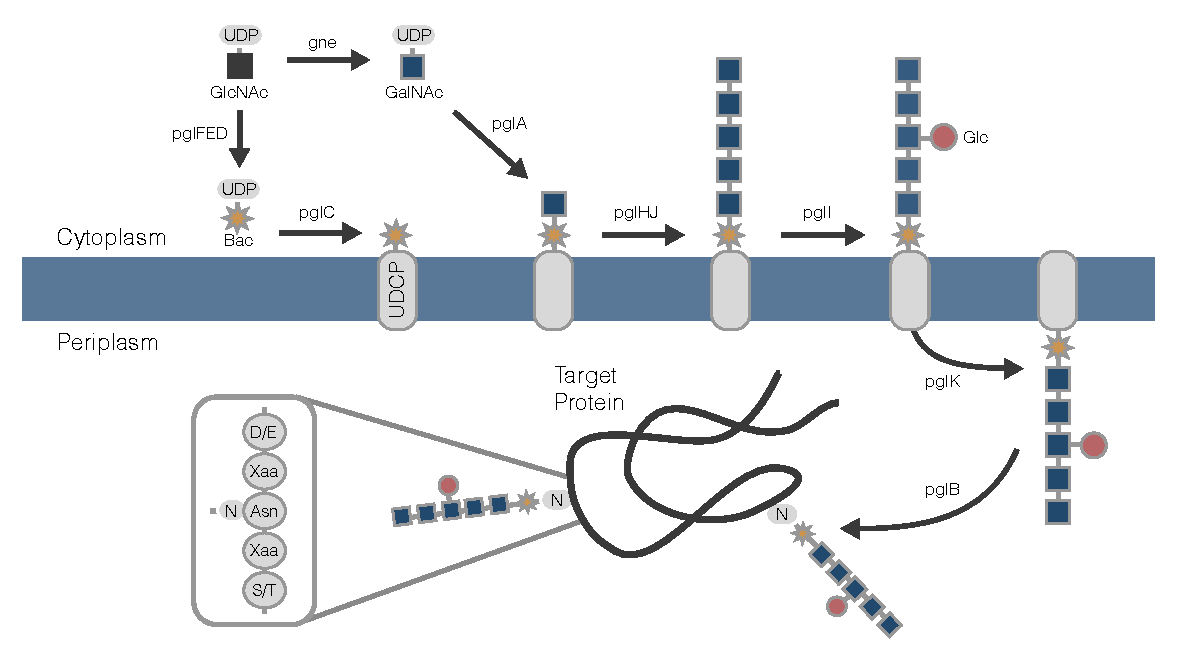
\includegraphics[width=1.0\textwidth]{./figures/fig1_glyco_pathway.pdf}
\caption{Glycosylation pathway in \textit{C. jejuni} and \textit{E. coli}. 
Glycan assembly, facilitated by \textit{pgl} locus enzymes, takes place on a lipid carrier, undecaprenyl pyrophosphate (UDCP), from cytoplasmic pools of nucleotide-activated sugars N-acetylglucosamine (GlcNAc), N-acetylgalactosamine (GalNAc), and glucose (Glc). 
The glycan is then flipped onto the periplasmic side of the inner membrane, where it is transferred to an asparagine residue on a glycoprotein acceptor motif.}
\label{fig_pathway_cjejuni}
\end{figure}

\clearpage

% Figure 2
\begin{figure}\centering
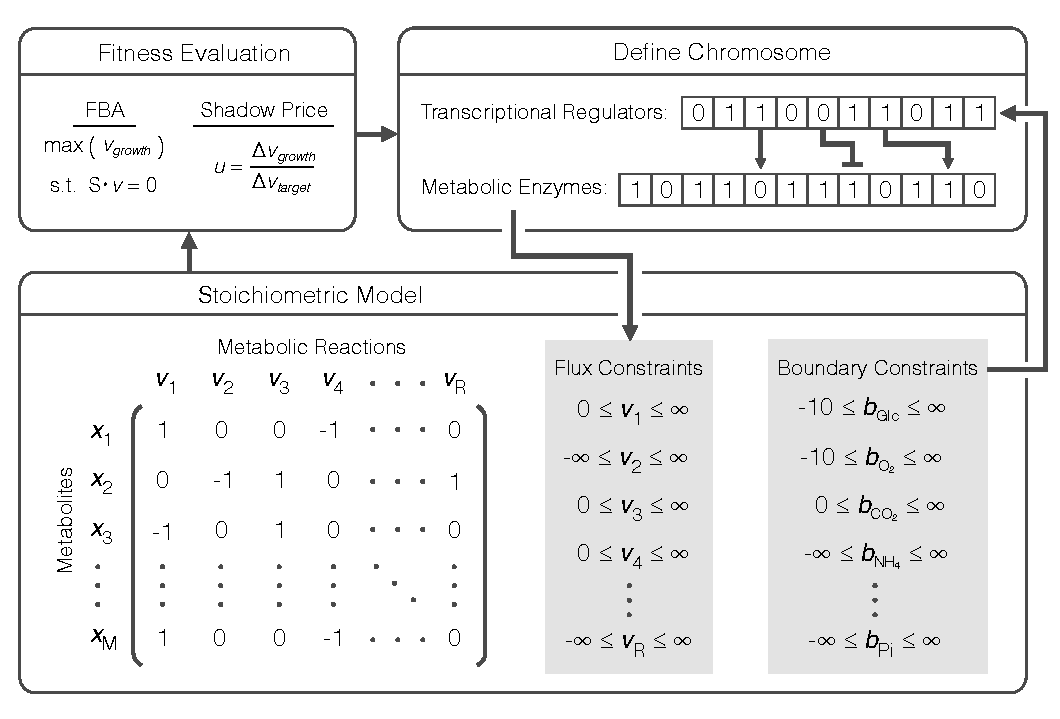
\includegraphics[width=1.0\textwidth]{./figures/fig2_workflow.pdf}
\caption{Heuristic optimization approach used to identify strains coupling growth to glycan production. 
The chromosome is defined as two separate binary arrays, one defining the state of metabolic enzyme expression and another defining the state of transcriptional regulator activation. 
Gene repression and knockouts are designated by zeros. 
Nutrient conditions define the boundary constraints within the stoichiometric model which in turn affect the state of the metabolic enzyme chromosome. 
Gene repression and knockouts determine the constraints placed on fluxes in the stoichiometric model. 
Nutrients are mapped to the state of transcriptional regulators and genes are mapped to the state of flux constraints using Boolean rules as defined in \cite{2004_covert_reed_herrgard_palsson_Nat,2007_feist_reed_hatzimanikatis_palsson_MolSysBio}. 
FBA is used to maximize growth rate under the constraints imposed by the mutant strain and transcriptional regulation and the fitness objective is calculated. 
Here, we use shadow price. 
The strain is accepted or rejected based on the change in fitness and a Boltzmann criterion. 
New mutant strains are randomly generated from accepted ones. 
The search continues until a positive shadow price is achieved.}
\label{fig_workflow_heuristic}
\end{figure}

\clearpage

% Figure 3
\begin{figure}\centering
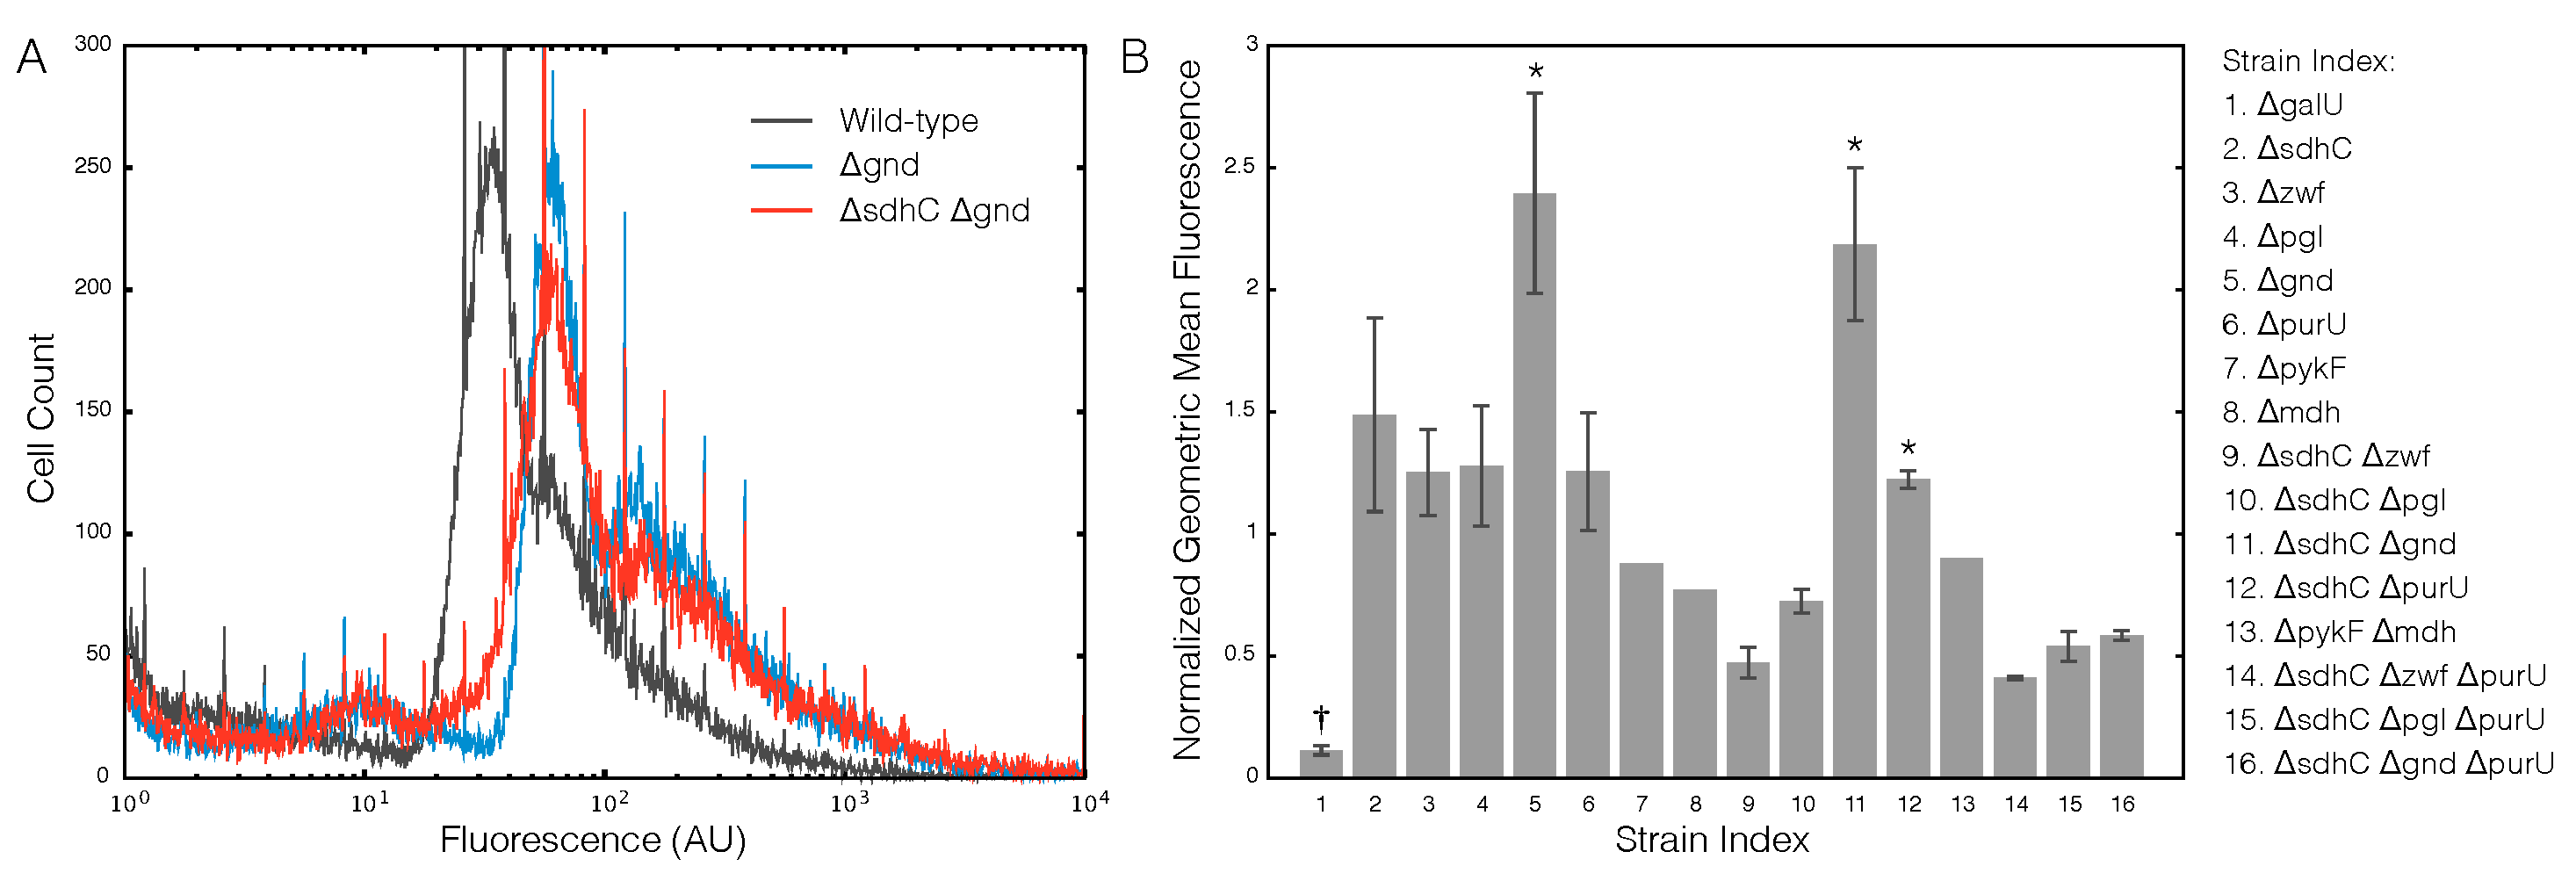
\includegraphics[width=1.0\textwidth]{./figures/fig3_FACS_hist.pdf}
\caption{\textbf{(A)} Fluorescence from outer membrane labeled \textit{C. jejuni} glycans of single knockout $\Delta$\textit{gnd} and double knockout $\Delta$\textit{sdhC} $\Delta$\textit{gnd}, detecting by flow cytometry. 
$\dagger$ indicates a strain predicted to eliminate glycan flux. 
Stars indicate statistically significant increases in fluorescence according to a t-test ($p<0.05$). 
\textbf{(B)} Geometric mean fluorescence, normalized to the wild-type value, from gene knockout strains appearing in growth-coupled strains identified by the constraint-based model. 
Error bars indicate the average of three replicates.}
\label{fig_FACS_all}
\end{figure}

\clearpage

% Figure 4
\begin{figure}\centering
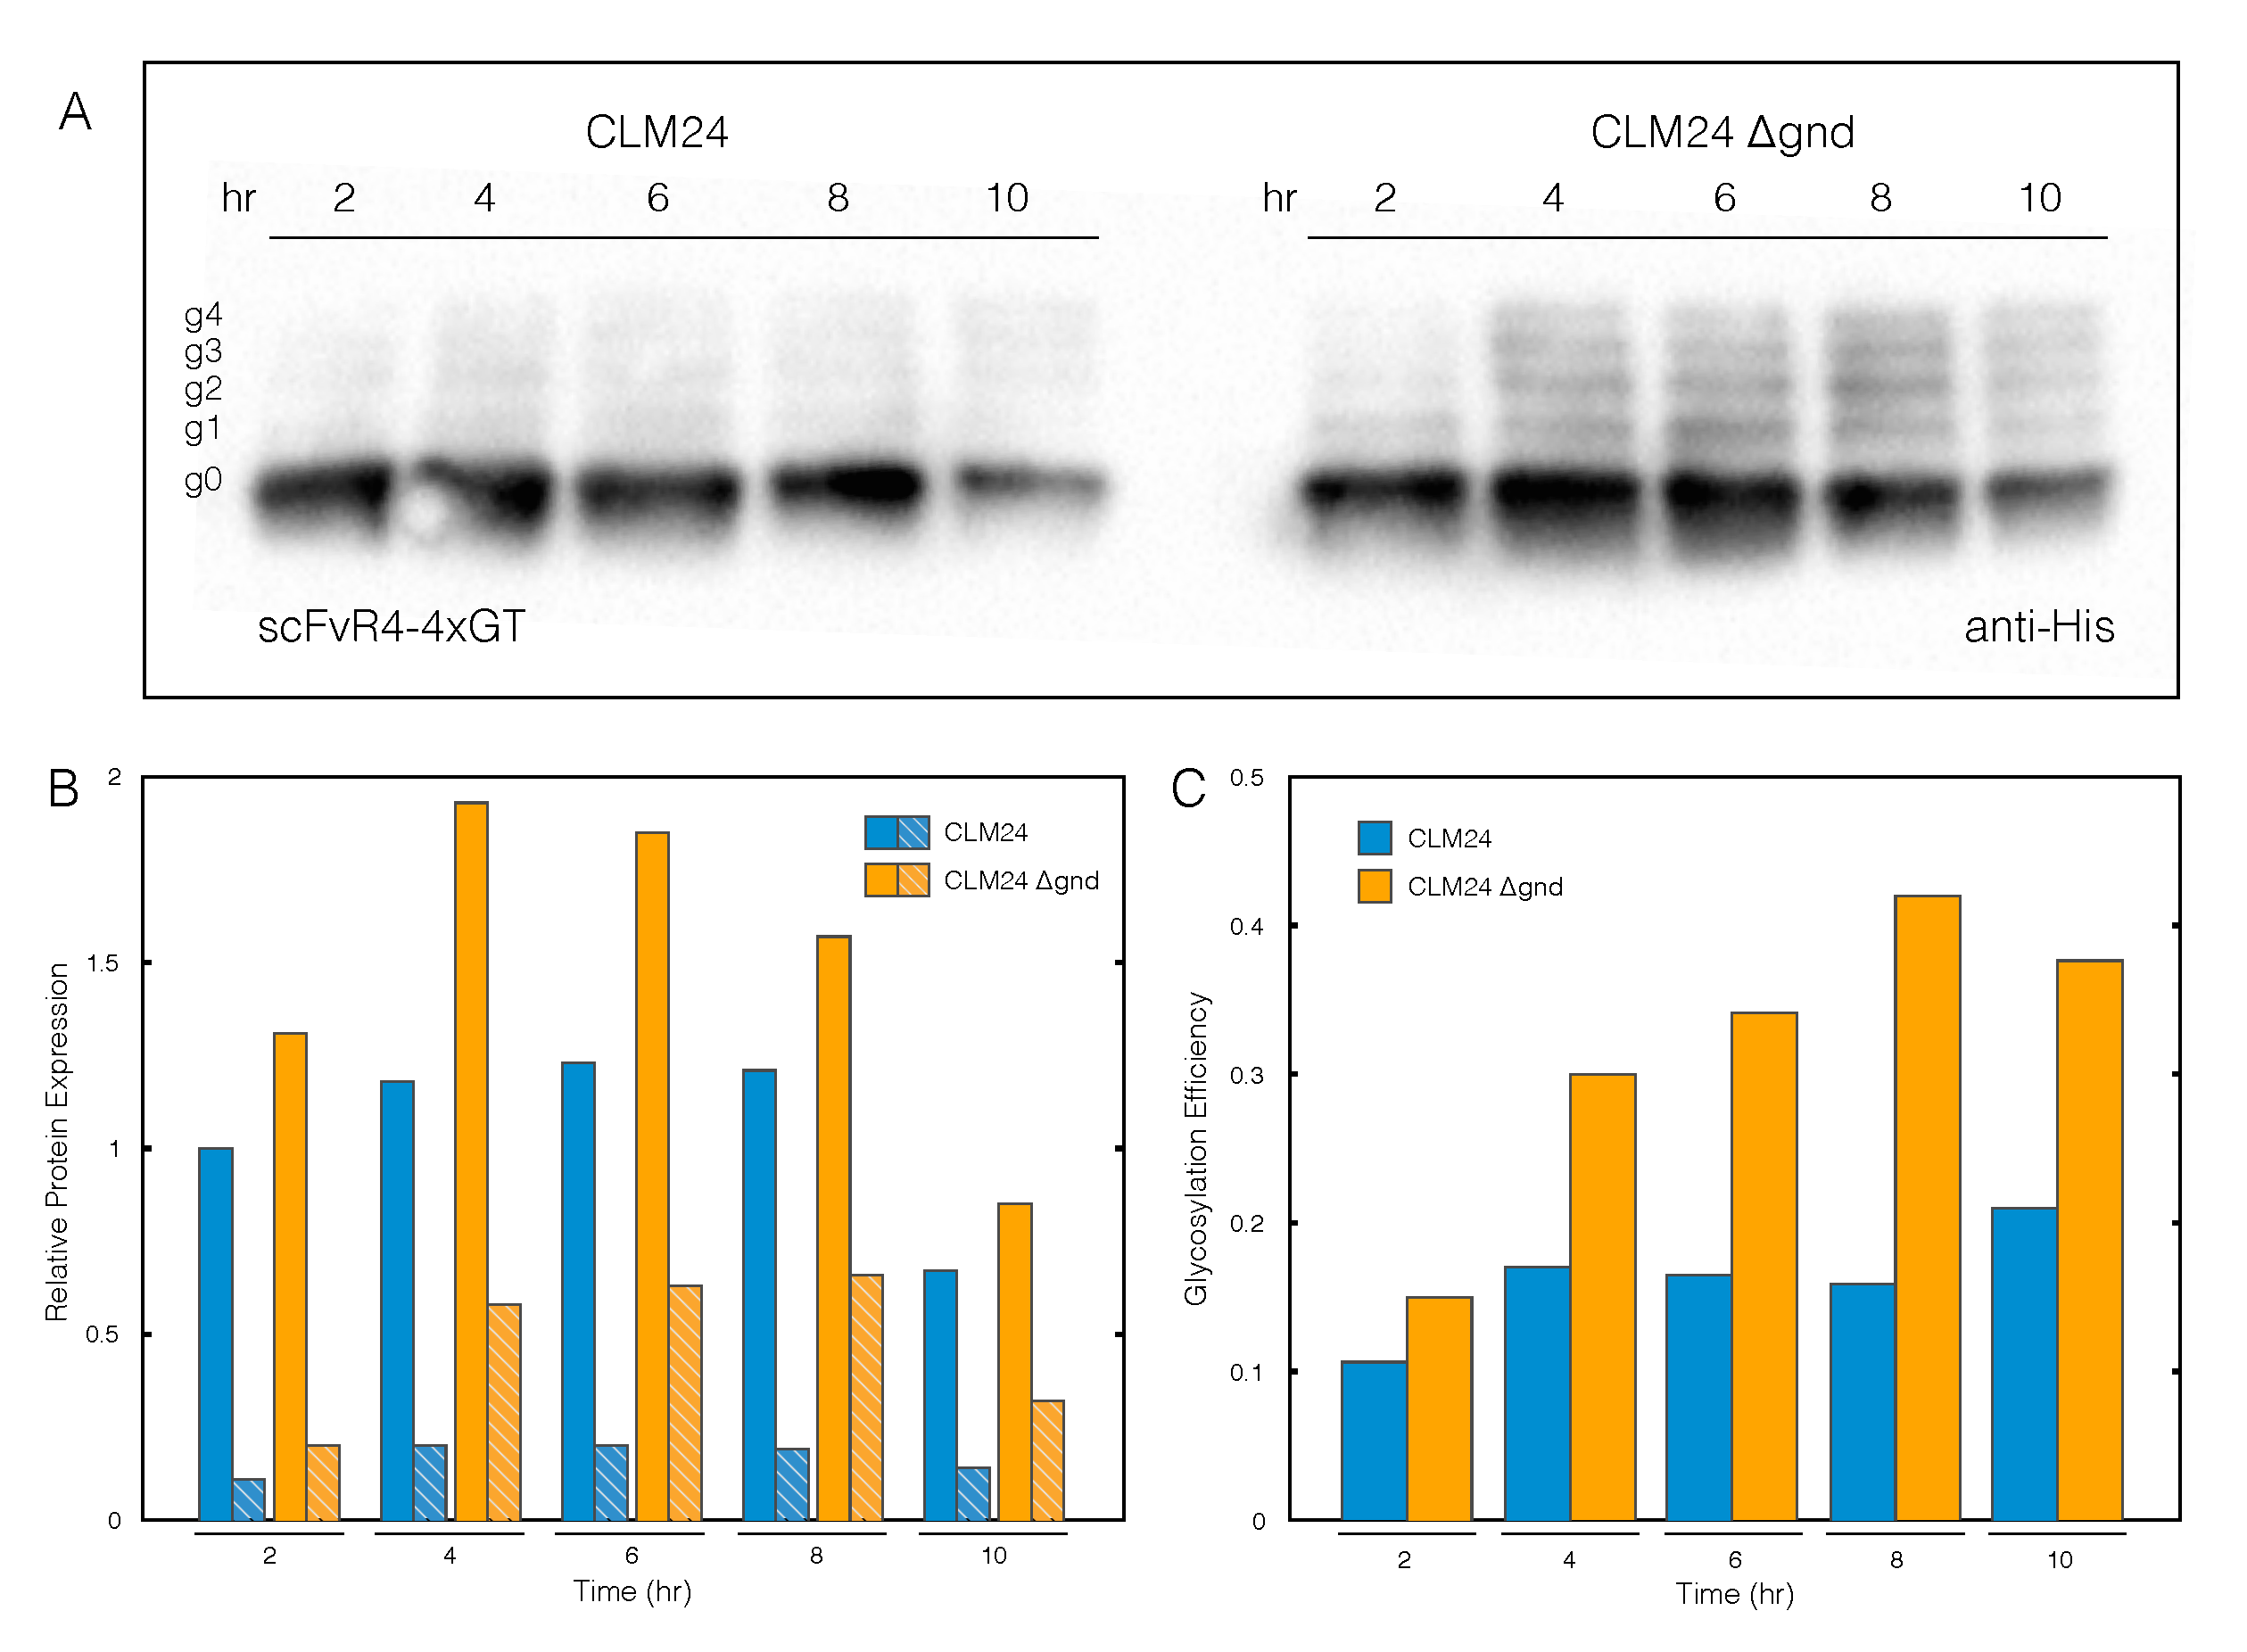
\includegraphics[width=1.0\textwidth]{./figures/fig4_western_gnd.pdf}
\caption{Western blot analysis of glycosylation efficiency in \textit{gnd} mutant. 
scFvR4 protein expression was induced during exponential growth phase. 
Time points indicate time after induction. 
\textbf{(A)} Relative protein expression over time. 
Striped bars indicate the portion of glycosylated protein. 
\textbf{(B)} Glycosylation efficiencies for each strain over time. 
Blot intensities were determined using image analysis software called ImageJ \cite{2012_schneider_eliceiri_NatMeth}.}
\label{fig_western_CLM24_gnd}
\end{figure}


%%%%%%%%%%%%%%%%%%%%%%%%%%%%%%%%%%%%%%%%%%%%%%%%%%%%%%%%%%%%%%%%%%%%%
% TABLES
%%%%%%%%%%%%%%%%%%%%%%%%%%%%%%%%%%%%%%%%%%%%%%%%%%%%%%%%%%%%%%%%%%%%%

\clearpage

% Table 1
\begin{center}
\tablefirsthead{
\hline
\rowcolor[gray]{0.8} Strain & Strain & Growth Rate & Glycan Flux \\
\rowcolor[gray]{0.8} Name & Genotype & (/hr) & (mmol/gDCW/hr) \\
\hline}
\topcaption{Wild-type along with growth-coupled strains producing \textit{C. jejuni} glycan identified by FBA and heuristic optimization. 
Simulations were performed with and without the transcription factor regulatory network. 
Knockouts listing multiple genes indicate that knockout of any one of those genes produces the same phenotype in the model. \\}
\label{tbl_sims_strains_KO}
\begin{scriptsize}
\begin{supertabular}{l l l l}
\\
Wild-type  &  & 0.78 & 0.0 \\
EcM1  & $\Delta$sdh $\Delta$zwf/pgl/gnd & 0.65 & 0.012 \\
EcM2  & $\Delta$sdh $\Delta$zwf/pgl/gnd $\Delta$pta $\Delta$eutD & 0.53 & 0.098 \\ 
EcM3  & $\Delta$sdh $\Delta$zwf/pgl/gnd $\Delta$pykAF $\Delta$mdh & 0.64 & 0.016 \\
EcM4$^\dagger$  & $\Delta$sdh $\Delta$zwf/pgl/gnd $\Delta$purU $\Delta$xdh/allABC & 0.65 & 0.007 \\
EcM5$^\dagger$  & $\Delta$sdh $\Delta$zwf/pgl/gnd $\Delta$purU $\Delta$xdh/allABC $\Delta$pta $\Delta$eutD & 0.58 & 0.055 \\
\\ \hline
  & $\dagger$ Strains without transcription factor regulation &  &  \\
\end{supertabular}
\end{scriptsize}
\end{center}

\end{document}
